\documentclass[12pt, a4paper]{article}
\usepackage[utf8]{inputenc}
\usepackage[russian]{babel}
\usepackage[pdftex]{graphicx, color}
\usepackage{amsmath, amsfonts, amssymb, amsthm}
\usepackage[left=2cm,right=2cm,top=1.5cm,bottom=2cm]{geometry}
\usepackage{indentfirst}

\usepackage{setspace}
\onehalfspacing
\graphicspath{{pics/}}

\begin{document}

    \thispagestyle{empty}

    \begin{singlespace}
    \begin{titlepage}
        \begin{center}
            
\includegraphics[height = 3cm]{msu.png}

            {\scshape Московский государственный университет имени М.~В.~Ломоносова}\\
            Факультет вычислительной математики и кибернетики\\
            Кафедра математических методов прогнозирования\\
            \centerline{\hfill\hrulefill\hrulefill\hrulefill\hrulefill\hfill}

            \vfill

            {\LARGE Отчет к первому практическому заданию по МОМО: \\ Точная одномерная оптимизация (вариант 1)}

            \vspace{1cm}

        \end{center}

        \vfill
        \begin{flushright}
            Студент 517 группы:\\
                \textit{Оспанов А.М.}

            \vspace{5mm}

        \end{flushright}

        \vfill

        \begin{center}
        Москва, 2016
        \end{center}
    \end{titlepage}
    \end{singlespace}

    \newpage
    \section{Введение}
        В данной работе будет реализован модуль optim1d.py с методами для одномерной оптимизации: метод ``Золотого сечения'', метод параболы, метод Брента, метод секущих и метод Брента с производной. Будут проведены исследования скоростей сходимости кажого метода и построены соответствующие графики. Также методы оптимизации без производной будут протестированы на многомодальных функциях.

        Код написан на языке Python с использованием библиотеки numpy.

    \section{Скорости сходимости методов}
        Скорости сходимости методов будут исследоваться на следующих функциях:
        \def \picwidth {14cm}
        \def \picheight {7.5cm}
        \begin{enumerate}
            \item $f(x) = -5 x^5 + 4 x^4 - 12 x^3 + 11 x^2 - 2 x + 1$ на интервале $[-0.5, 0.5]$
                \begin{center}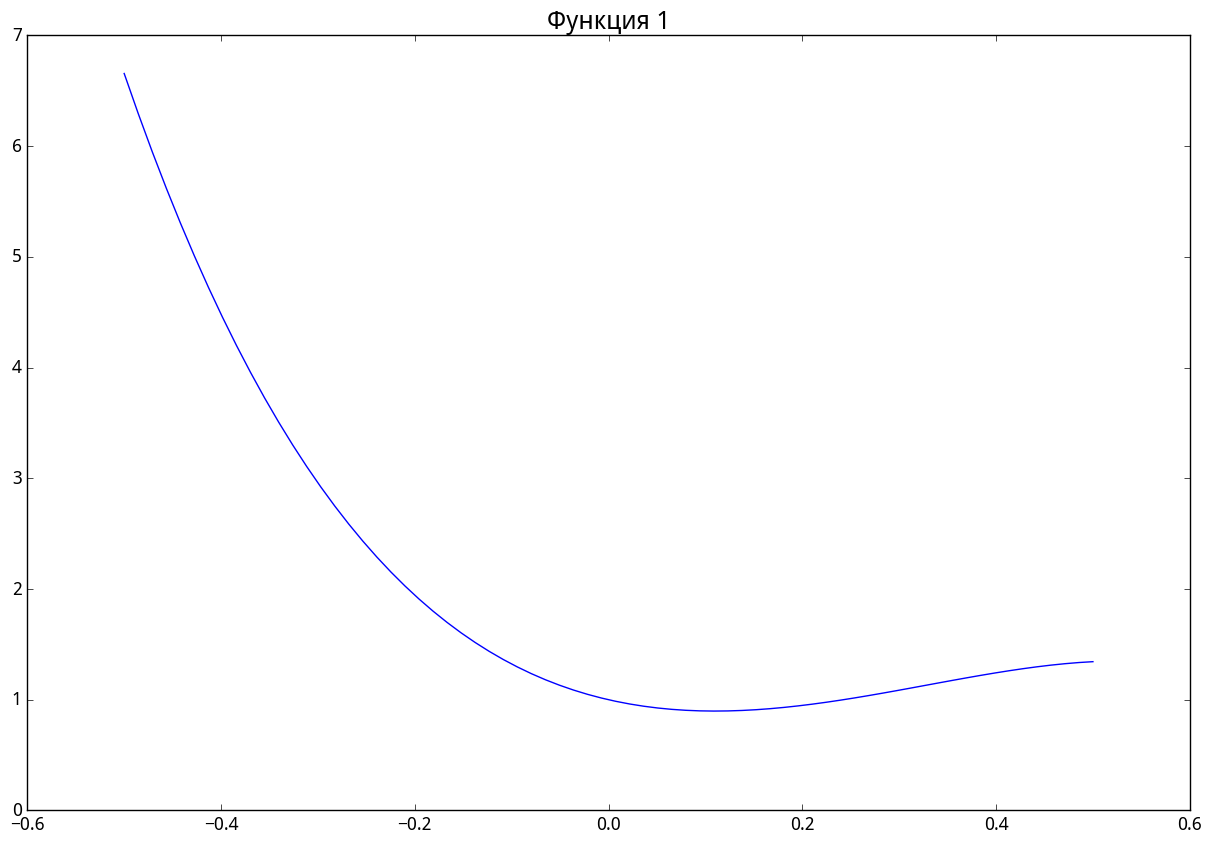
\includegraphics[width=\picwidth, height=\picheight]{fun1.png}\end{center}

            \item $f(x) = -ln^2(x - 2) + ln^2(10 - x) - x^{0.2}$ на интервале $[6, 9.9]$
                \begin{center}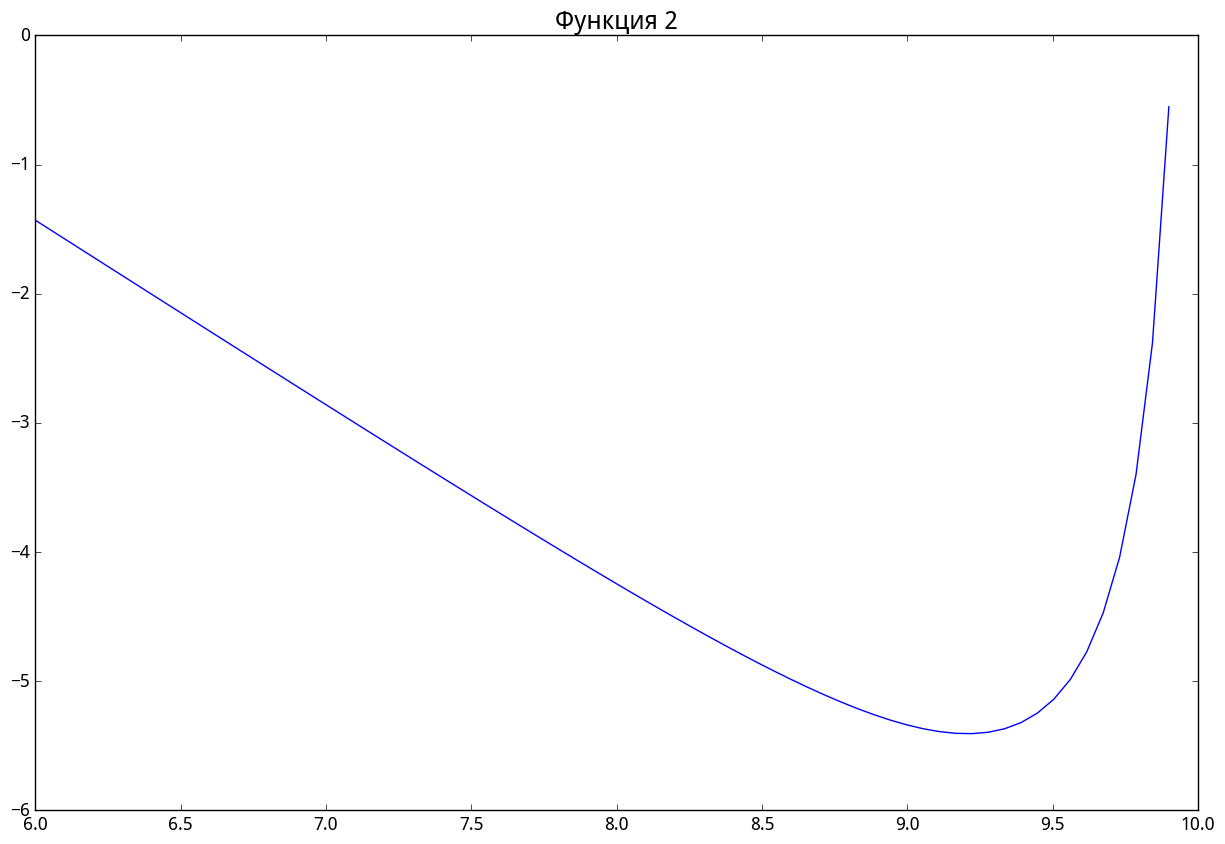
\includegraphics[width=\picwidth, height=\picheight]{fun2.png}\end{center}

            \item $f(x) = -3x sin(0.75x) + exp(-2x)$ на интервале $[0, 2\pi]$
                \begin{center}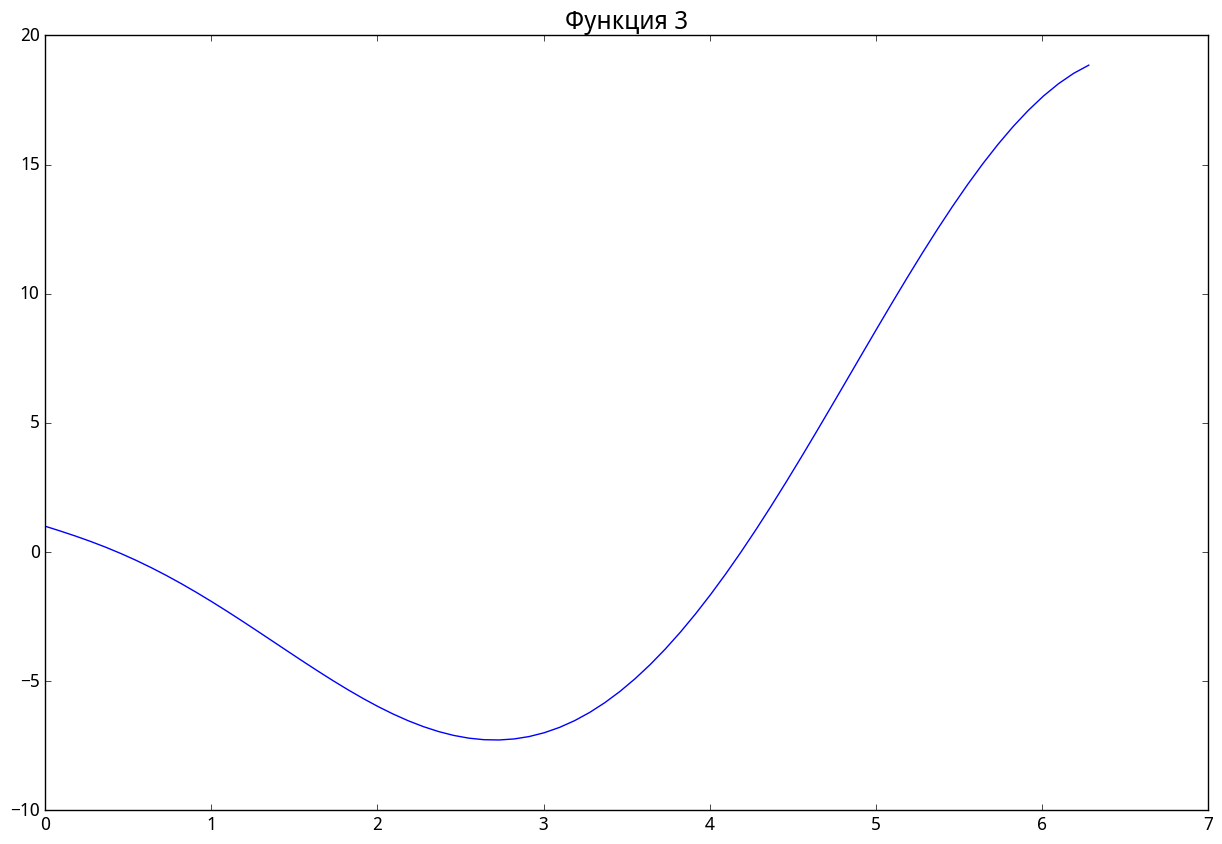
\includegraphics[width=\picwidth, height=\picheight]{fun3.png}\end{center}

            \item $f(x) = exp(3x) + 5 exp(-2x)$ на интервале $[0, 1]$
                \begin{center}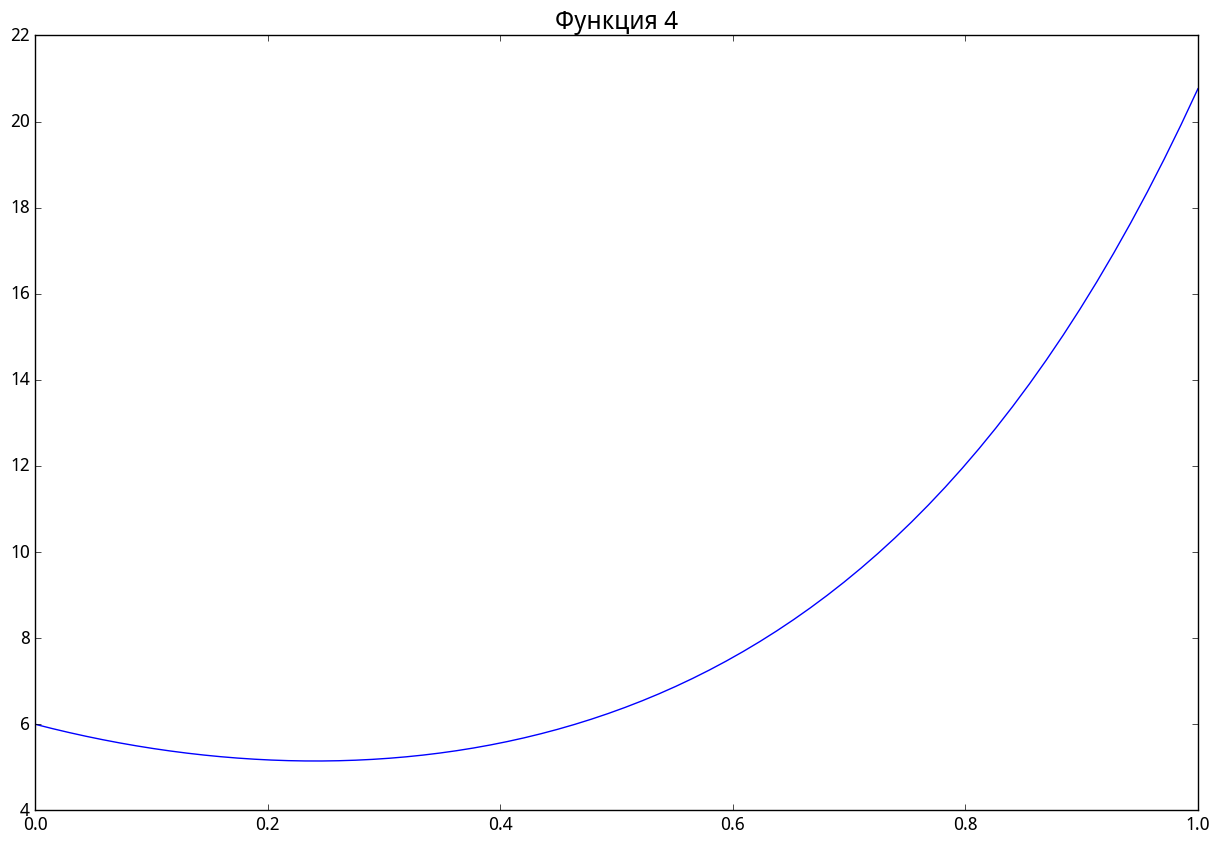
\includegraphics[width=\picwidth, height=\picheight]{fun4.png}\end{center}

            \item $f(x) = 0.2x ln x + (x - 2.3)^2$ на интервале $[0.5, 2.5]$
                \begin{center}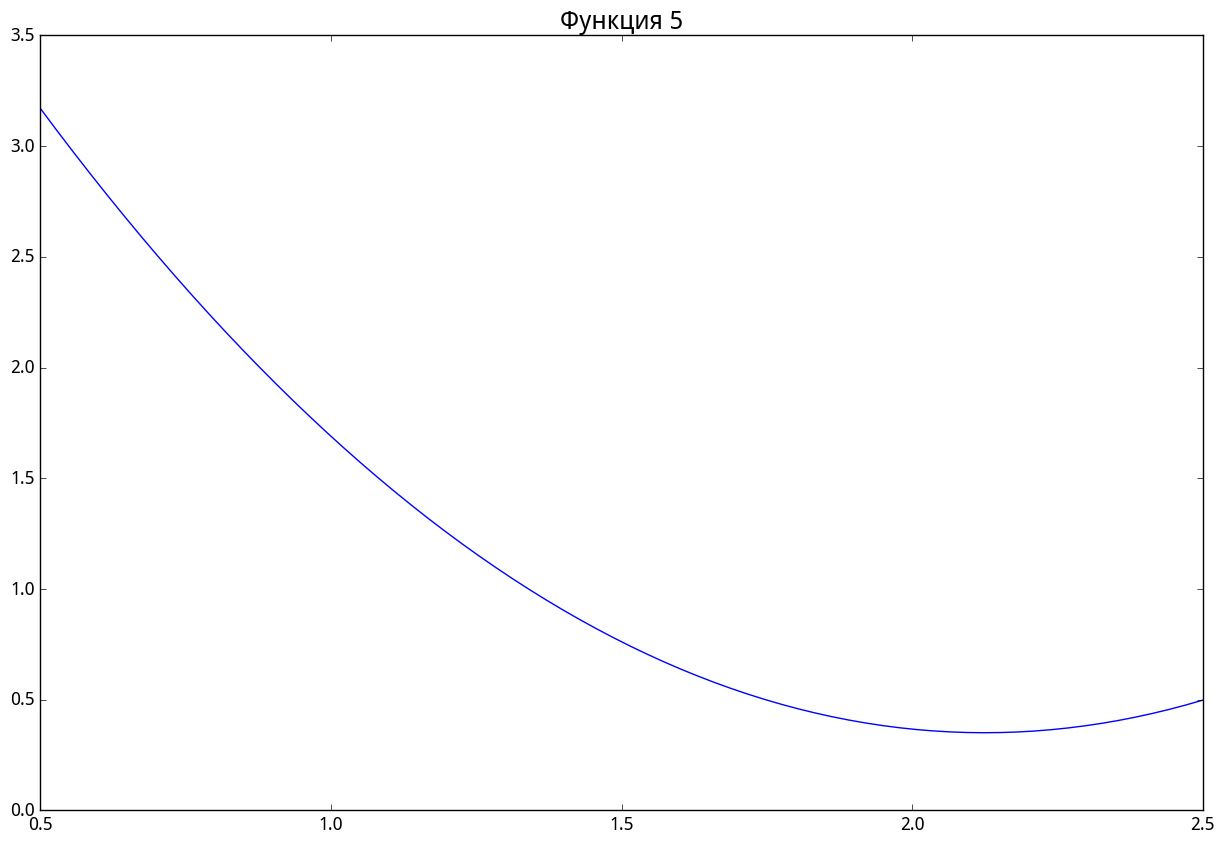
\includegraphics[width=\picwidth, height=\picheight]{fun5.png}\end{center}

        \end{enumerate}

        Рассмотрим скорости сходимости методов без производной.
        \def \picwidth {15.2cm}

        \textbf{Функция 1}

        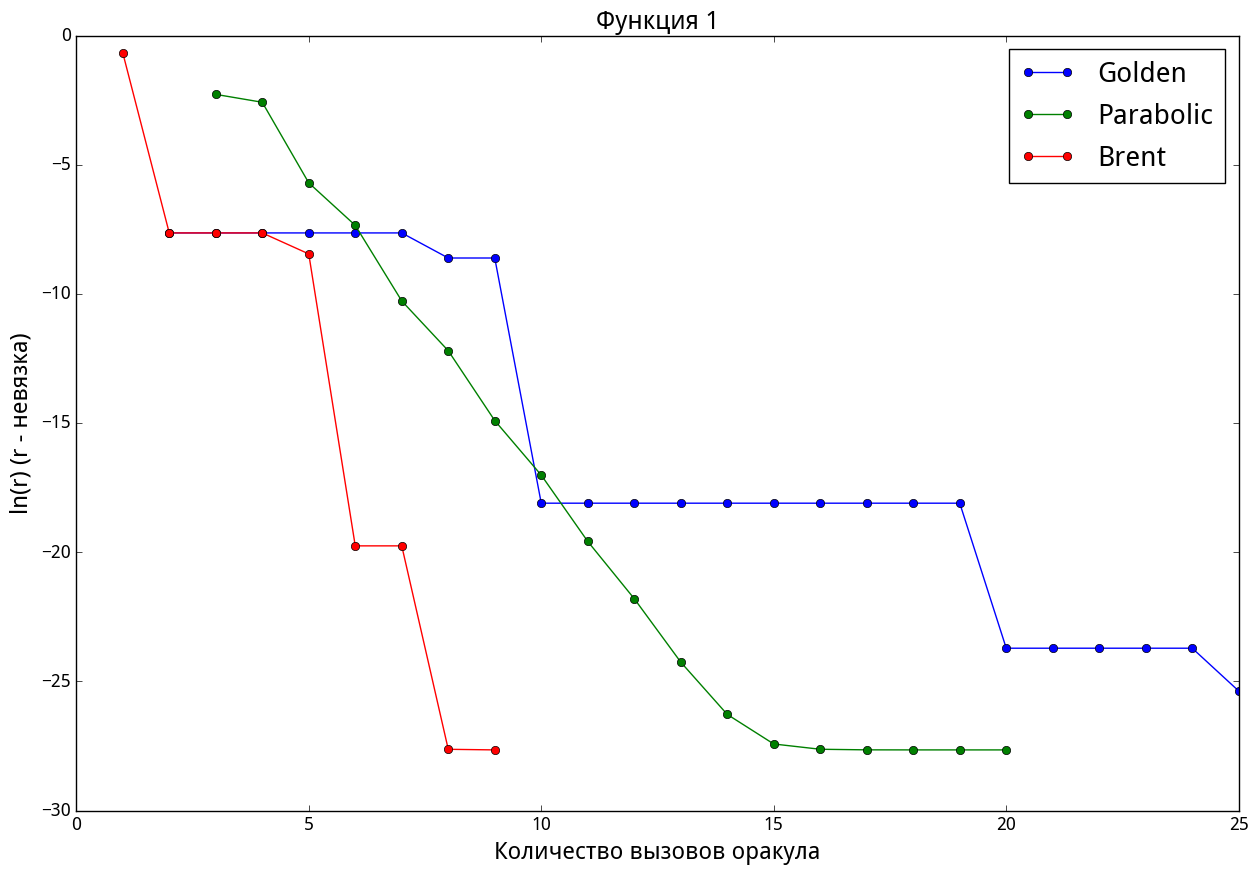
\includegraphics[width=\picwidth]{pics/fun1_nonder.png}

        На графике для первой функции видно, что метод ``Золотого сечения'' (ЗС) при некоторой апроксимации сходится линейно. Метод параболы сходится сублинейно. А с методом Брента не все ясно, похоже и на суперлинейную и на линейную сходимость. Рассмотрим его на дальнейших графиках.

        \textbf{Функция 2}

        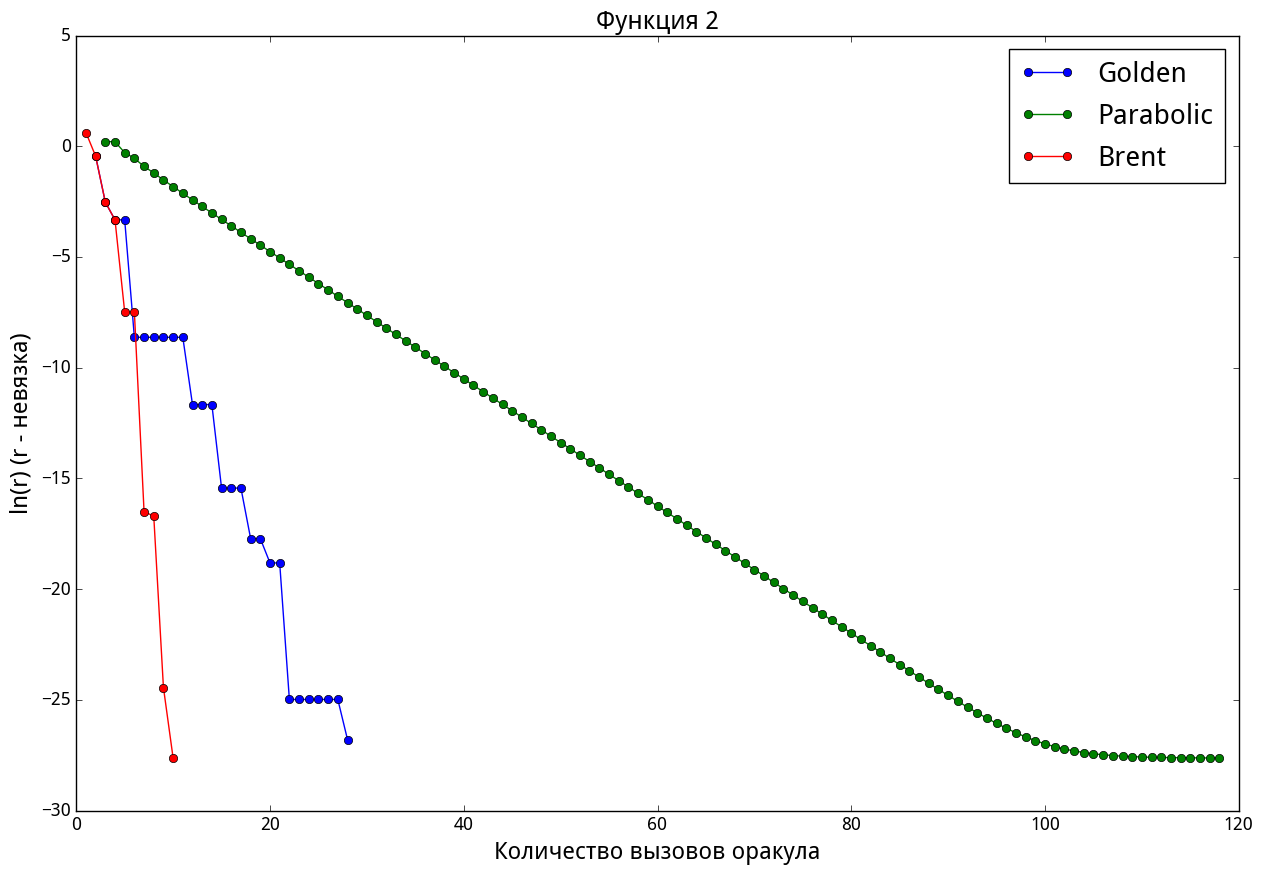
\includegraphics[width=\picwidth]{pics/fun2_nonder.png}

        На графике для второй функции видно, что метод ЗС сходится линейно, а метод параболы сходится сублинейно. А с методом Брента тут все очевидно и он сходится суперлинейно.

        Также на графике видно, что метод параболы сходится медленно, но это уже специфика функции. Функция 2 плохо аппроксимируется параболой, что приводит к медленной сходимости.

        \textbf{Функция 3}

        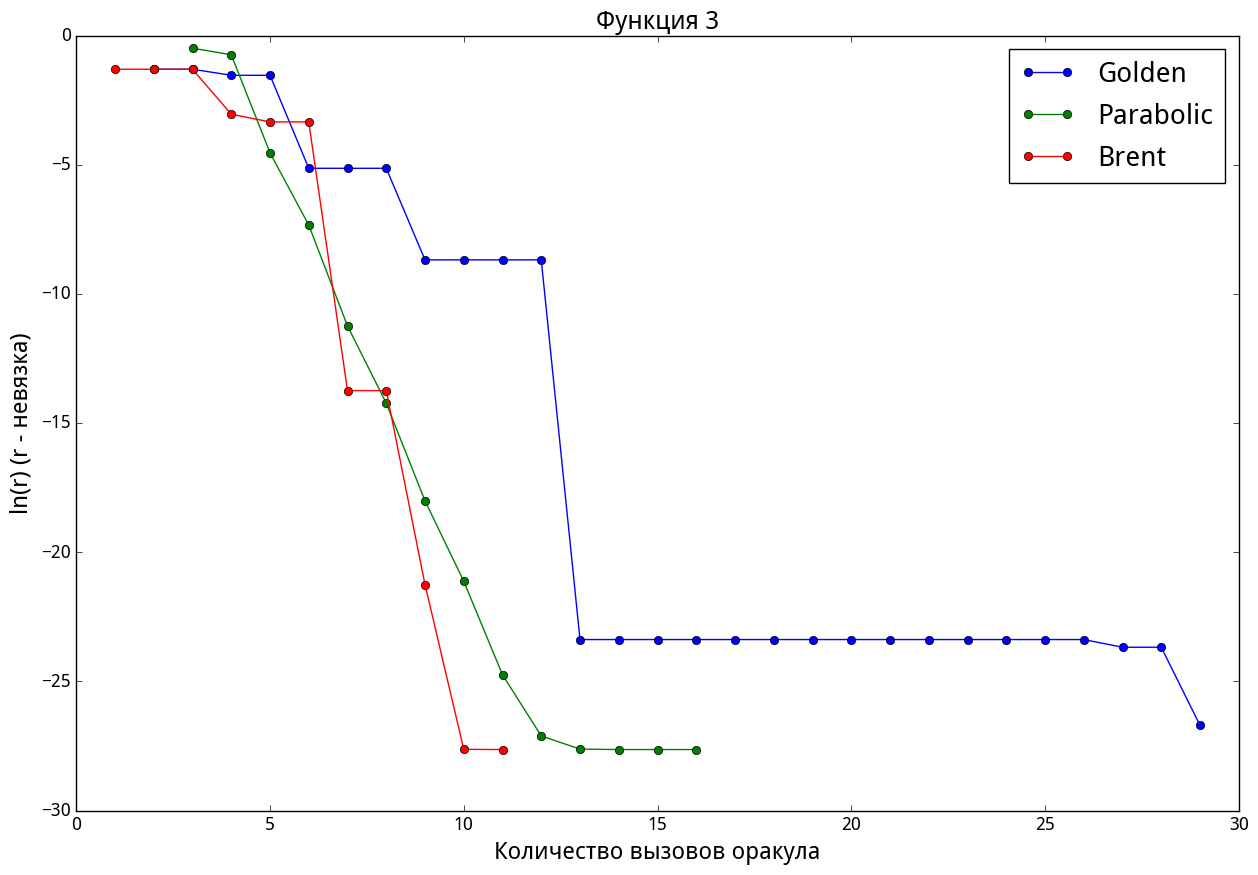
\includegraphics[width=\picwidth]{pics/fun3_nonder.png}

        \textbf{Функция 4}

        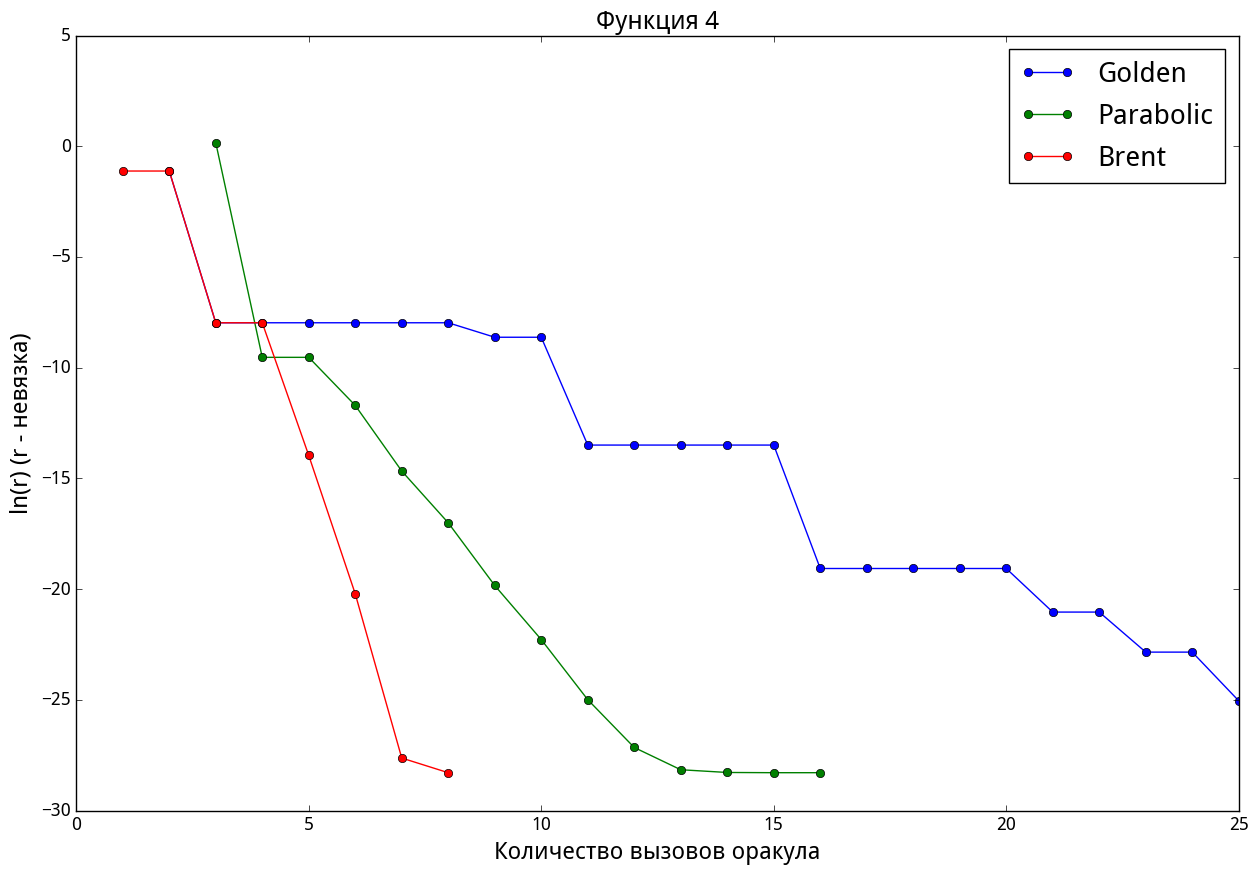
\includegraphics[width=\picwidth]{pics/fun4_nonder.png}

        \textbf{Функция 5}

        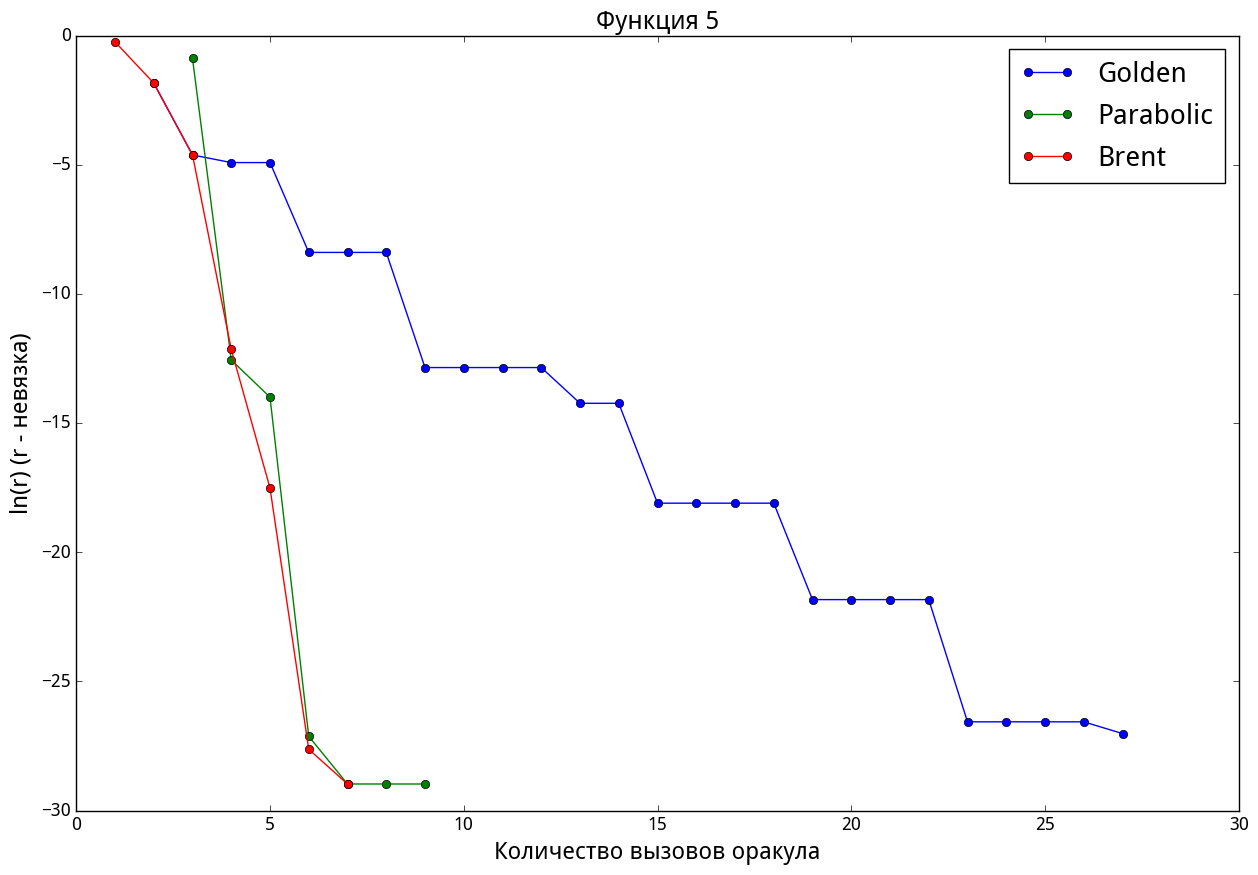
\includegraphics[width=\picwidth]{pics/fun5_nonder.png}

        Графики для 3-5 функций практический аналогичны и на них видно то же, что и на первых 2-х: скорости сходимости методов такие же.

        В итоге можно сделать вывод о том, что метод ЗС имеет линейную скорость сходимости, метод парабол - сублинейную и метод Брента - суперлинейную скорость сходимости.


    \section{Минимизация многомодальных функций}
        В качестве многомодальной функции рассмотрим $f(x) = sin(x)$ на разных интервалах.

        \def \picwidth {17cm}
        \def \picheight {7.8cm}

        \textbf{Интервал $[\pi, 4\pi]$} (Начальная точка метода параболы на максимуме)

        \begin{center}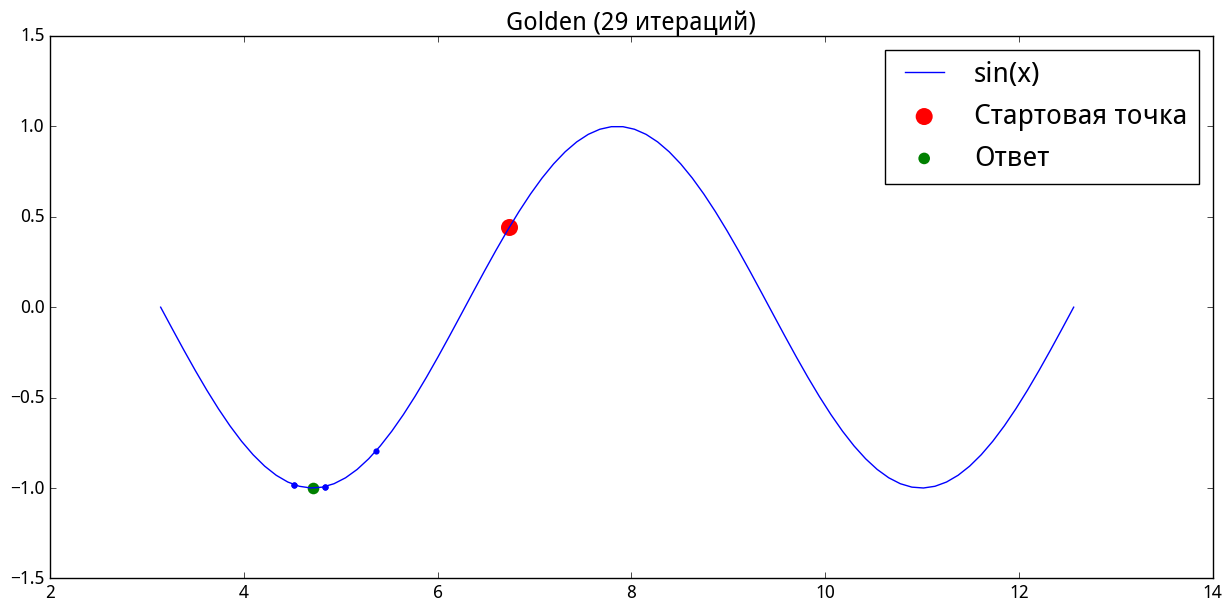
\includegraphics[width=\picwidth, height=\picheight]{pics/sin_golden_4p.png}\end{center}

        Метод золотого сечения на многомодальных функциях ведет себя как ``мячик с минимальной горизонтальной инерцией''. Т.е. в сторону какого минимума подтолкнешь, тот минимум и найдет.

        \begin{center}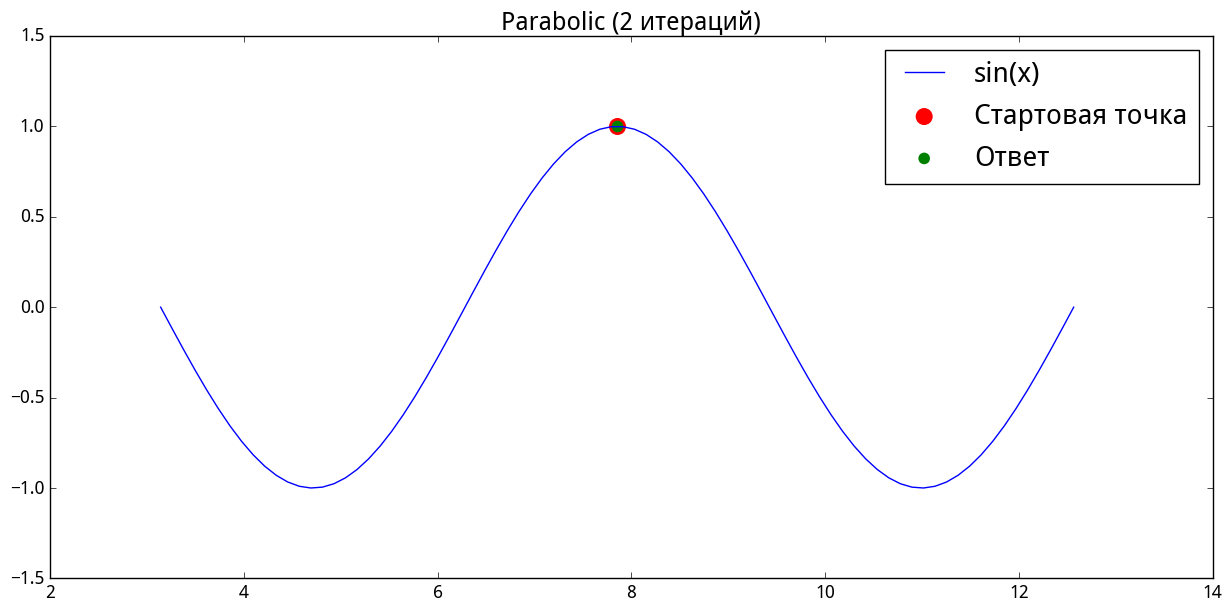
\includegraphics[width=\picwidth, height=\picheight]{pics/sin_parabolic_4p.png}\end{center}

        С параболой все не так. Тут видно, что парабола застревает в точке старта. Это связано с тем, что экстремум (на этом графике максимум) построенной параболы находится в этой же точке. Соответственно мы находим локальный максимум функции.

        \begin{center}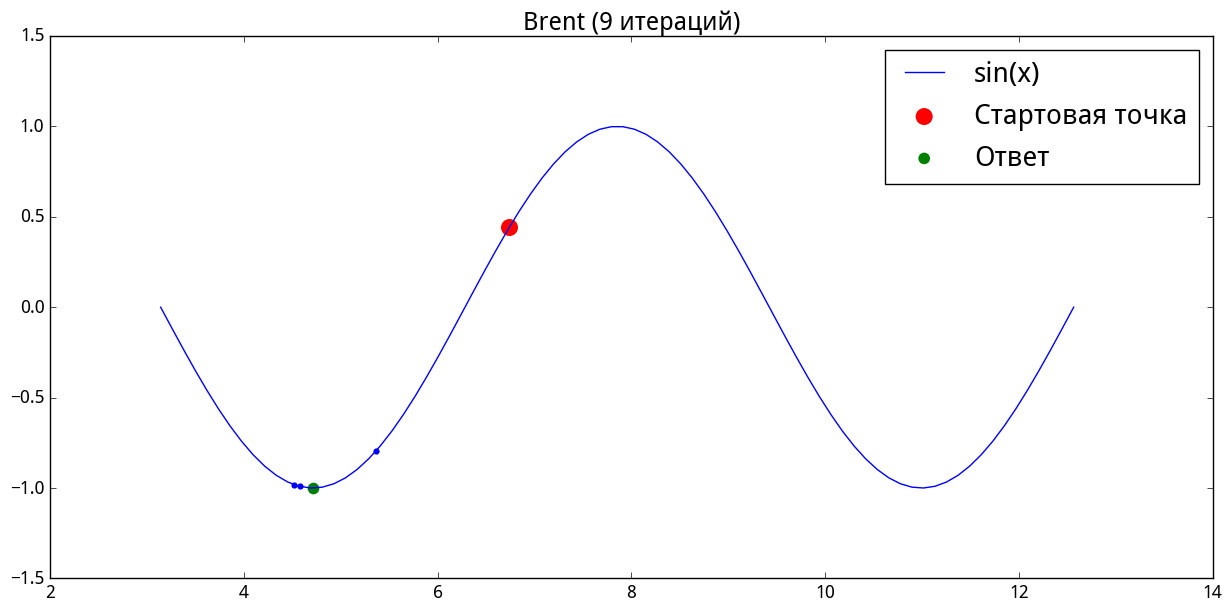
\includegraphics[width=\picwidth, height=\picheight]{pics/sin_brent_4p.png}\end{center}

        С Брентом все проще. Т.к. метод Брента содержит метод ЗС, то мы не застреваем на максимуме и работаем примерно как тот же ``мячик'', но быстрее благодаря методу парабол. (9 итераций против 29 в методе ЗС)



        \textbf{Интервал $[\pi, 7\pi]$}

        На данном интервале нам интересен результат метода парабол. Метод парабол на данном интервале сходится, т.к. начальная точка $(a + b) / 2$ не совпадает с локальным максимумом и соотвественно не застревает там же. Остальные методы ведут себя так же.

        \begin{center}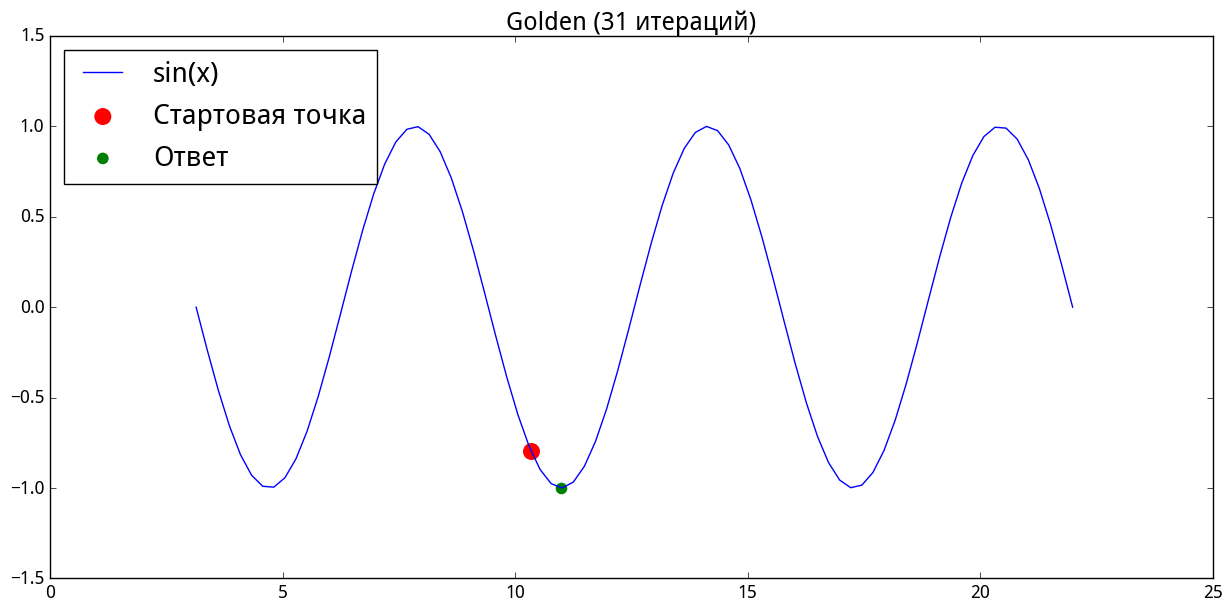
\includegraphics[width=\picwidth, height=\picheight]{pics/sin_golden_7p.png}\end{center}

        \begin{center}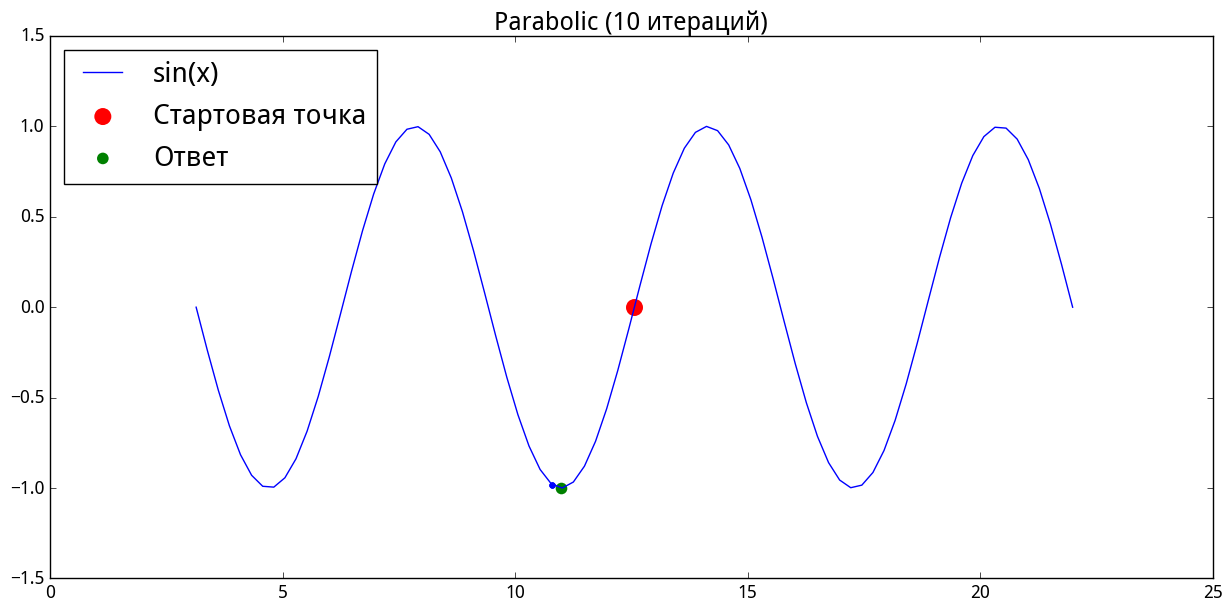
\includegraphics[width=\picwidth, height=\picheight]{pics/sin_parabolic_7p.png}\end{center}

        \begin{center}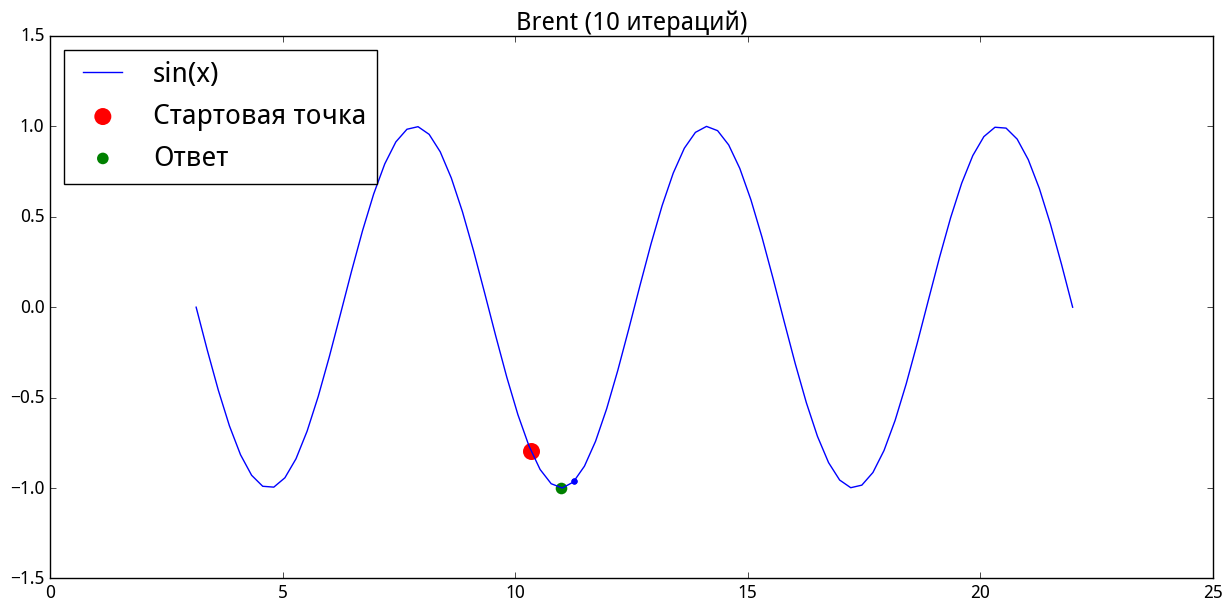
\includegraphics[width=\picwidth, height=\picheight]{pics/sin_brent_7p.png}\end{center}



        \textbf{Интервал $[\pi, 4.927\pi]$} (Начальная точка метода Брента на максимуме)

        \begin{center}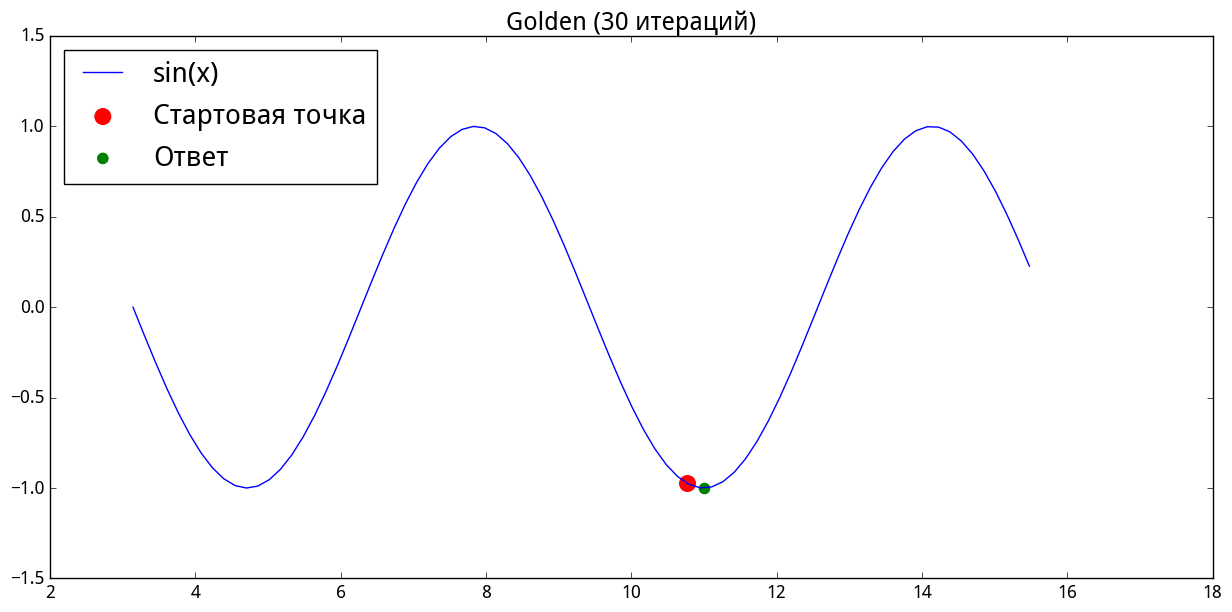
\includegraphics[width=\picwidth, height=\picheight]{pics/sin_golden_gp.png}\end{center}

        Метод ЗС также хорошо сходится.

        \begin{center}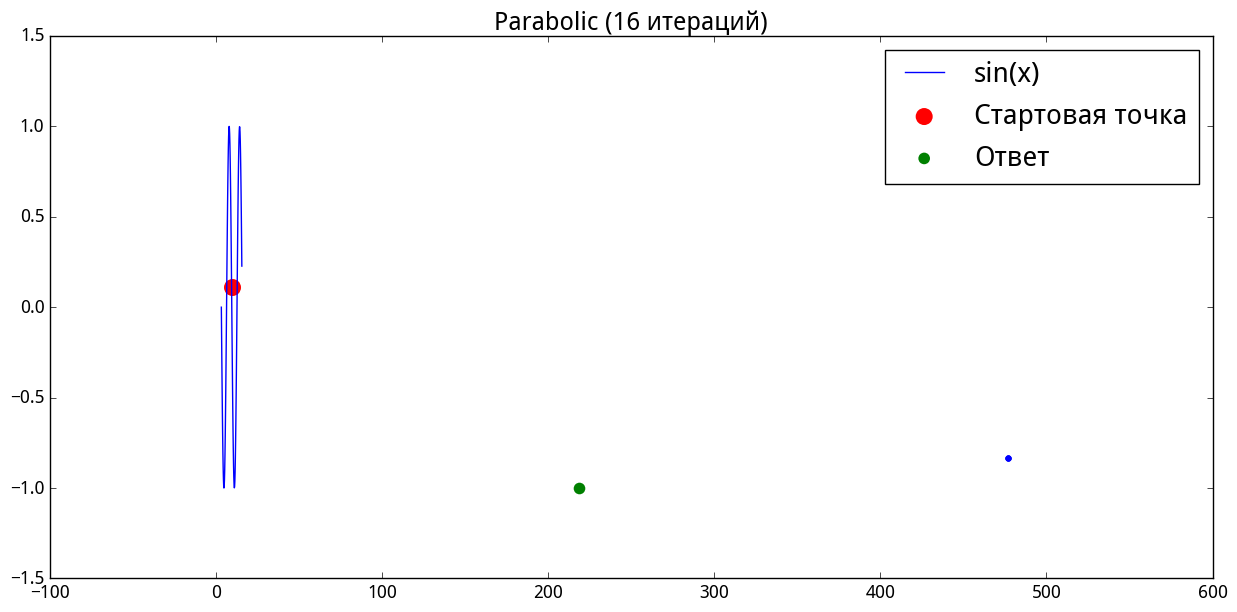
\includegraphics[width=\picwidth, height=\picheight]{pics/sin_parabolic_gp.png}\end{center}

        А вот метод парабол повел себя непредсказуемо. Вроде бы метод должен был сойтись в левый минимум, но вместо этого сошелся в минимум за интервалом. Это случилось по причине того, что начальная точка лежит не ниже, чем крайние точки.

        \begin{center}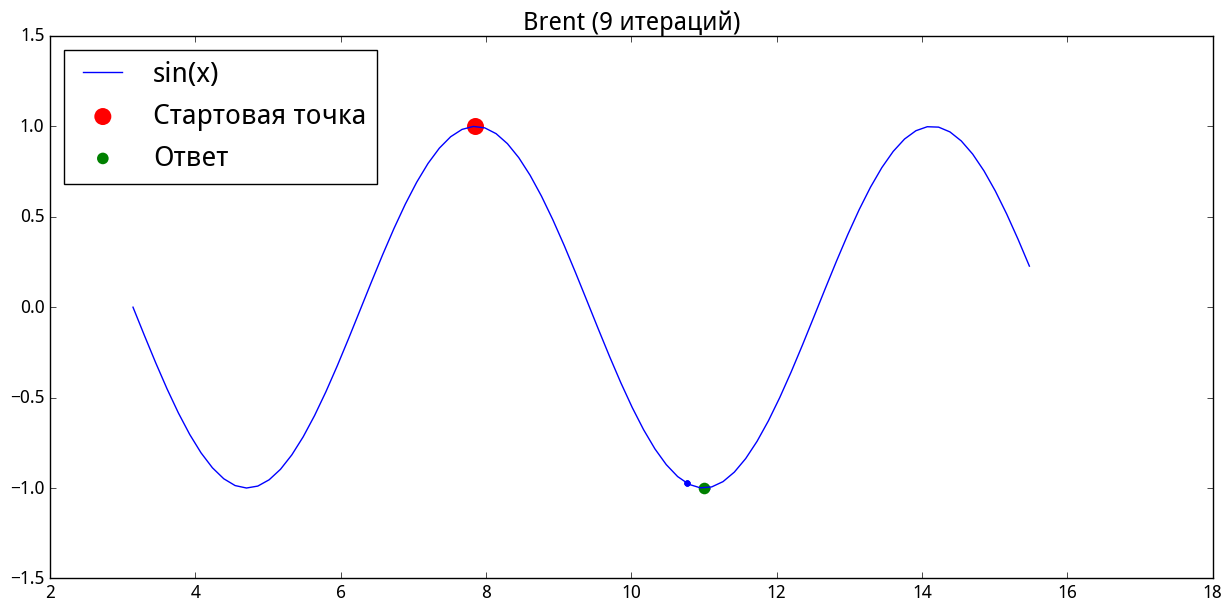
\includegraphics[width=\picwidth, height=\picheight]{pics/sin_brent_gp.png}\end{center}

        Метод Брента сходится даже при условии, что начальная точка совпадает с точкой максимума. Это происходит благодаря составляющей метода - ЗС, т.к. именно метод ЗС работает в данном случае.

        В итоге можно сделать вывод, что метод ЗС сойдется на многомодальных функциях к одному из локальных минимумов как и метод Брента. А метод парабол ведет себя непредсказуемо на таких функциях.

        Давайте теперь попробуем ответить на вопрос ``Могут ли методы золотого сечения/Брента вместо локального минимума найти локальный максимум или седловую точку и почему?''.

        Метод ЗС может найти седловую точку. Это может случиться, если средние две точки попадут на седловую точку и метод уйдет в сторону от минимума. Но в общем случае это маловероятно. А максимум метод не найдет, т.к. метод всегда стремится минимизировать функцию, т.е. берет минимум по двум средним точкам, что не позволит найти максимум. Приведем пример:

        \[ F(x) =
        \begin{cases}
            x^2       & \quad \text{если } x < 0 \\
            0         & \quad \text{если } 0 \leq x < 5 \\
            x^2 - 12 x + 35 & \quad \text{if } x \geq 5 \\
        \end{cases}
        \]

        \begin{center}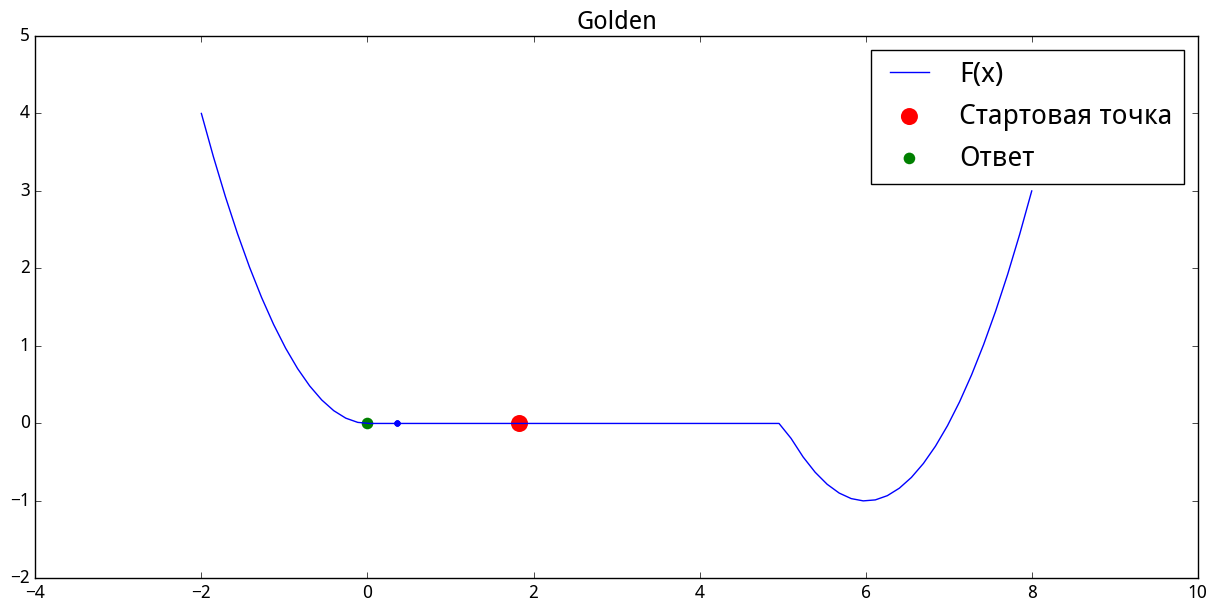
\includegraphics[width=\picwidth, height=\picheight]{pics/spec_func_golden.png}\end{center}

        Как видно из верхнего графика, метод ЗС после нахождения двух средних точек, выбрал левую и дальше рассматривал левую часть функции, т.е. ``ушел'' от минимума.

        Метод Брента не имеет ни одной из минусов, т.к. сочетает в себе два метода, которые не позволяет найти ни максимум, ни седловую точку. Посмотрим на той же функции, как поведет себя метод Брента

        \begin{center}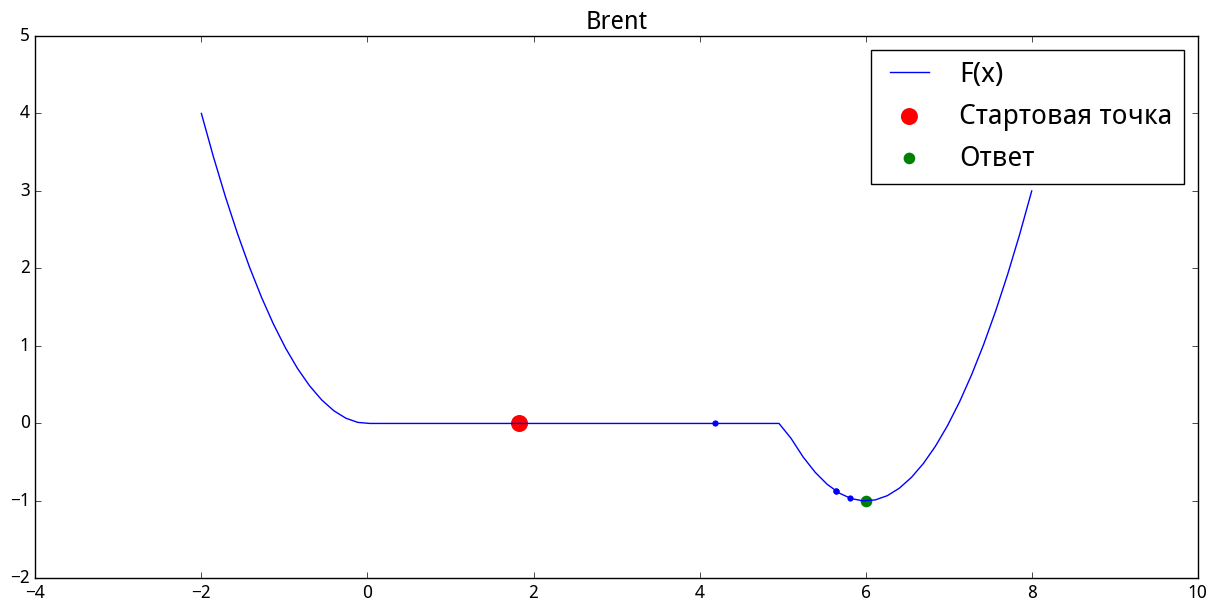
\includegraphics[width=\picwidth, height=\picheight]{pics/spec_func_brent.png}\end{center}

        Видим, что все работает хорошо, и метод Брента сошелся. Также стоит отметить, что метод сошелся за 8 шагов, 4 из которых сделал метод парабол. И к тому же, метод парабол для данной задачи тоже застрял в седловой точке. Это говорит о том, что метод Брента хоть и содрежит методы, находящие седловую точку, но благодаря хорошему их сочетанию, работает без застреваний.

        В итоге метод ЗС может найти седловую точку, но в очень редких случаях. Метод Брента сходится всегда.

    \section{Скорости сходимости методов с производной}
        Рассмотрим скорости сходимости методов c производной и сравним с методами без производной.
        \def \picwidth {15.8cm}

        \textbf{Функция 1}

        \begin{center}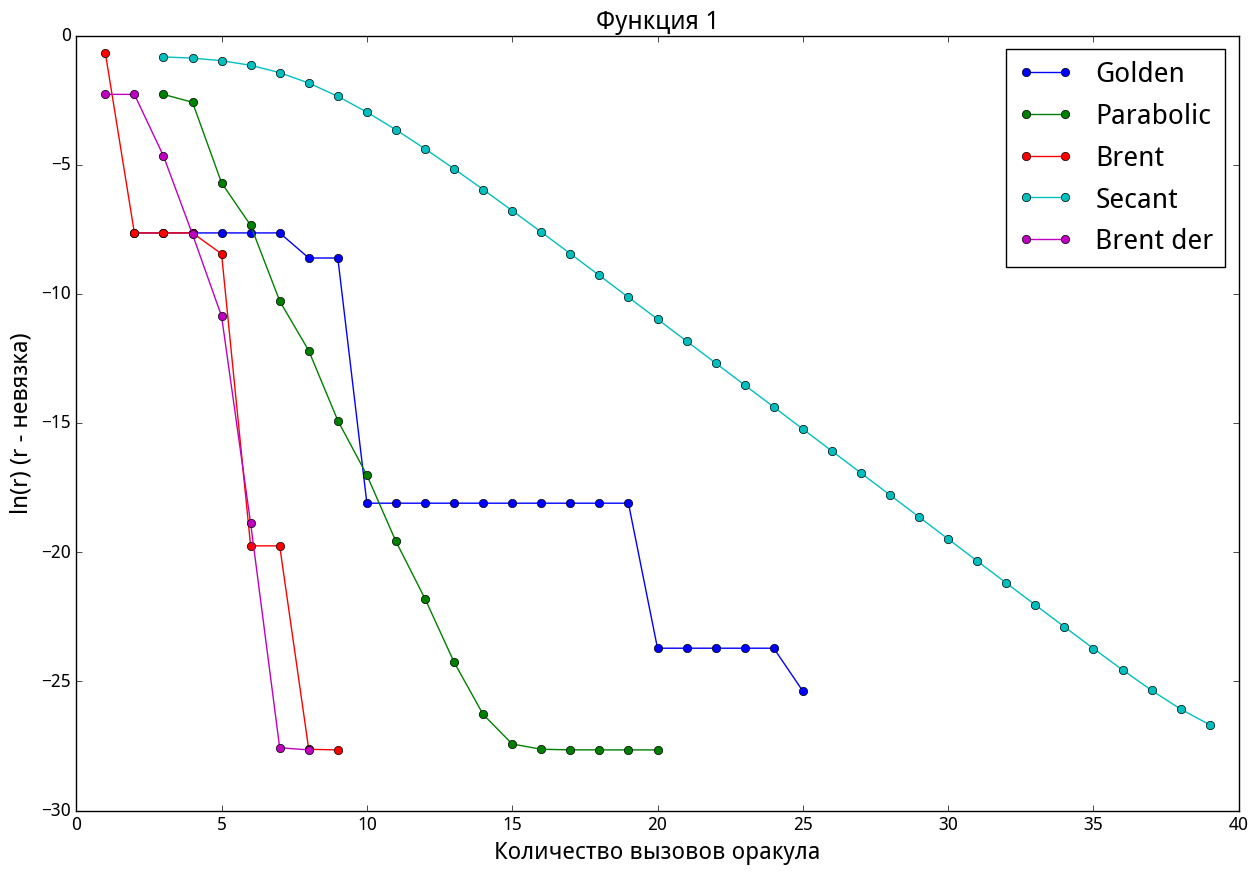
\includegraphics[width=\picwidth]{pics/fun1_der.png}\end{center}

        \textbf{Функция 2}

        \begin{center}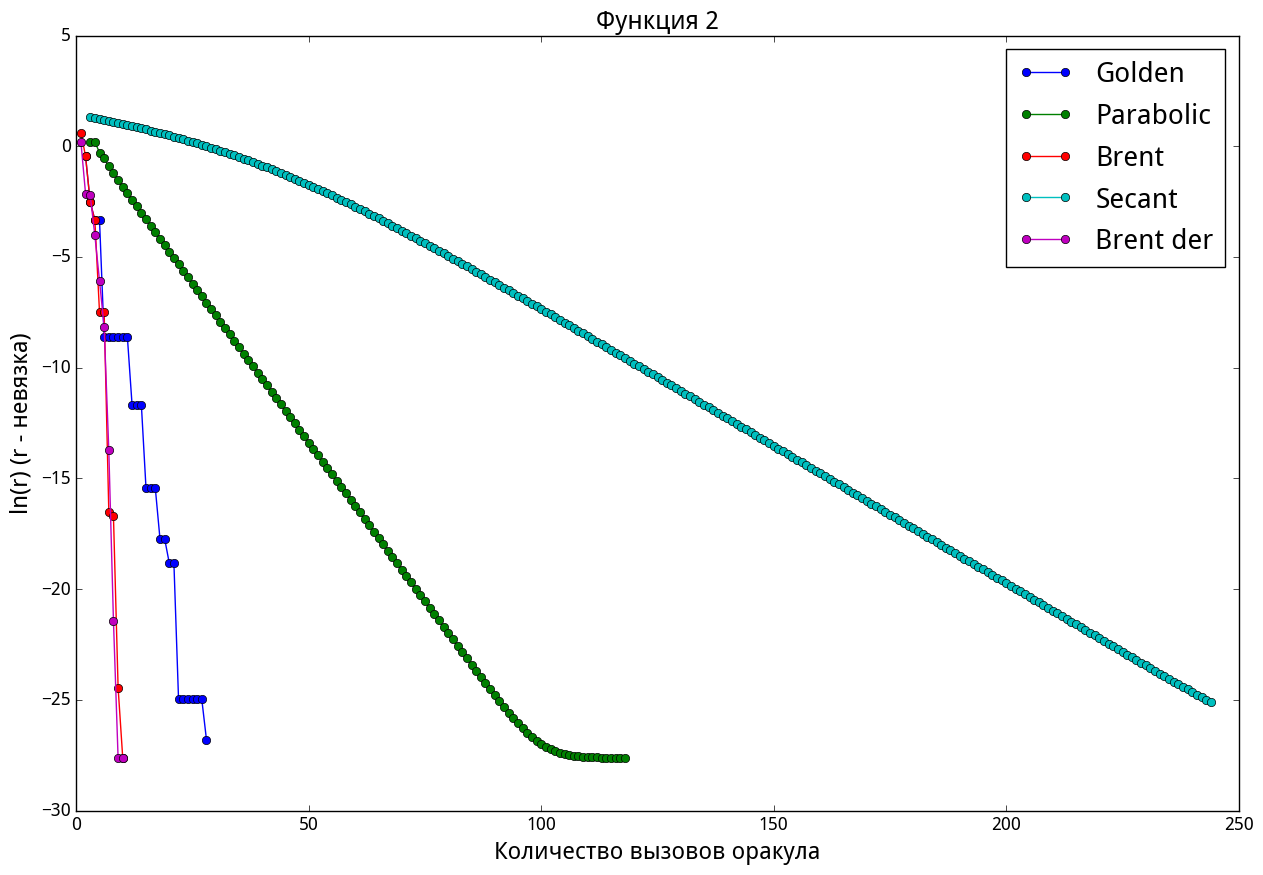
\includegraphics[width=\picwidth]{pics/fun2_der.png}\end{center}

        \textbf{Функция 3}

        \begin{center}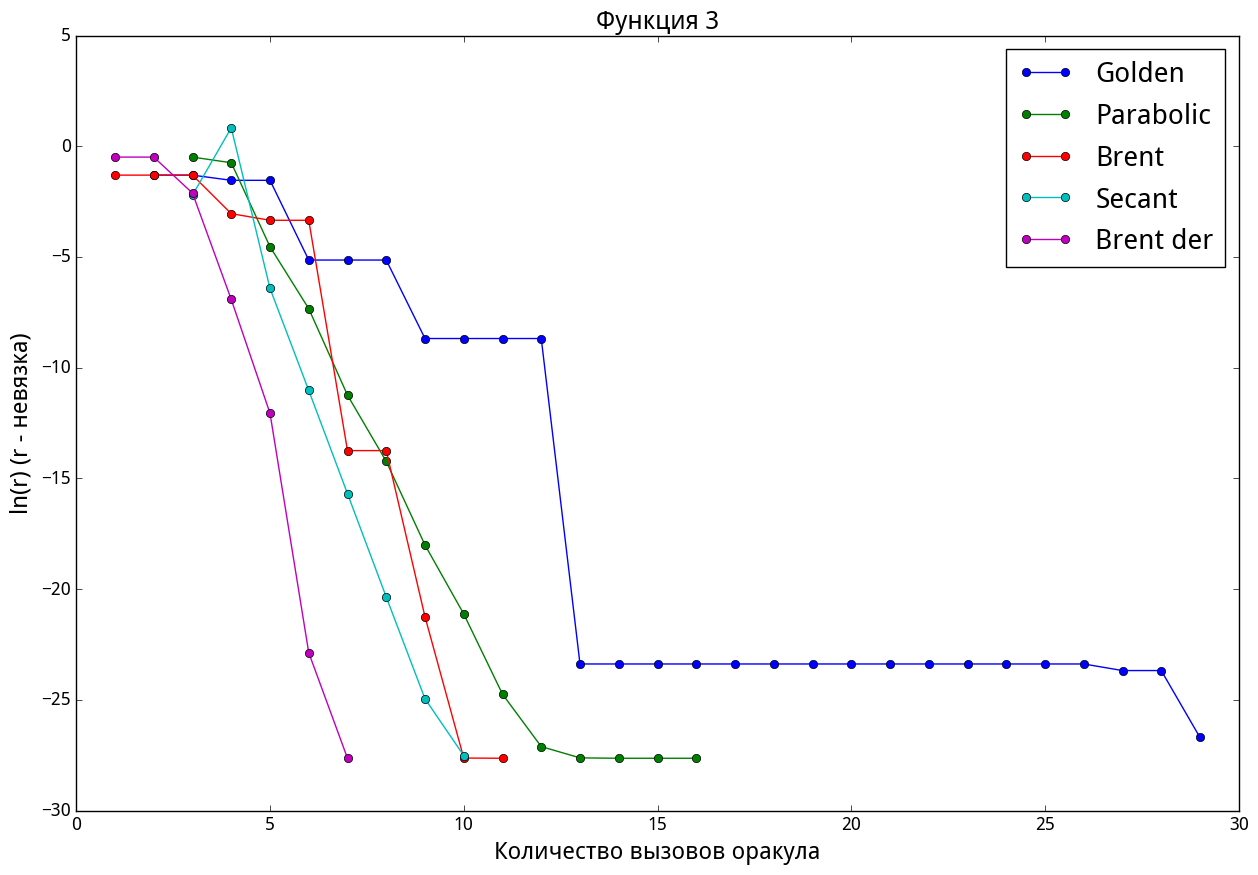
\includegraphics[width=\picwidth]{pics/fun3_der.png}\end{center}

        \textbf{Функция 4}

        \begin{center}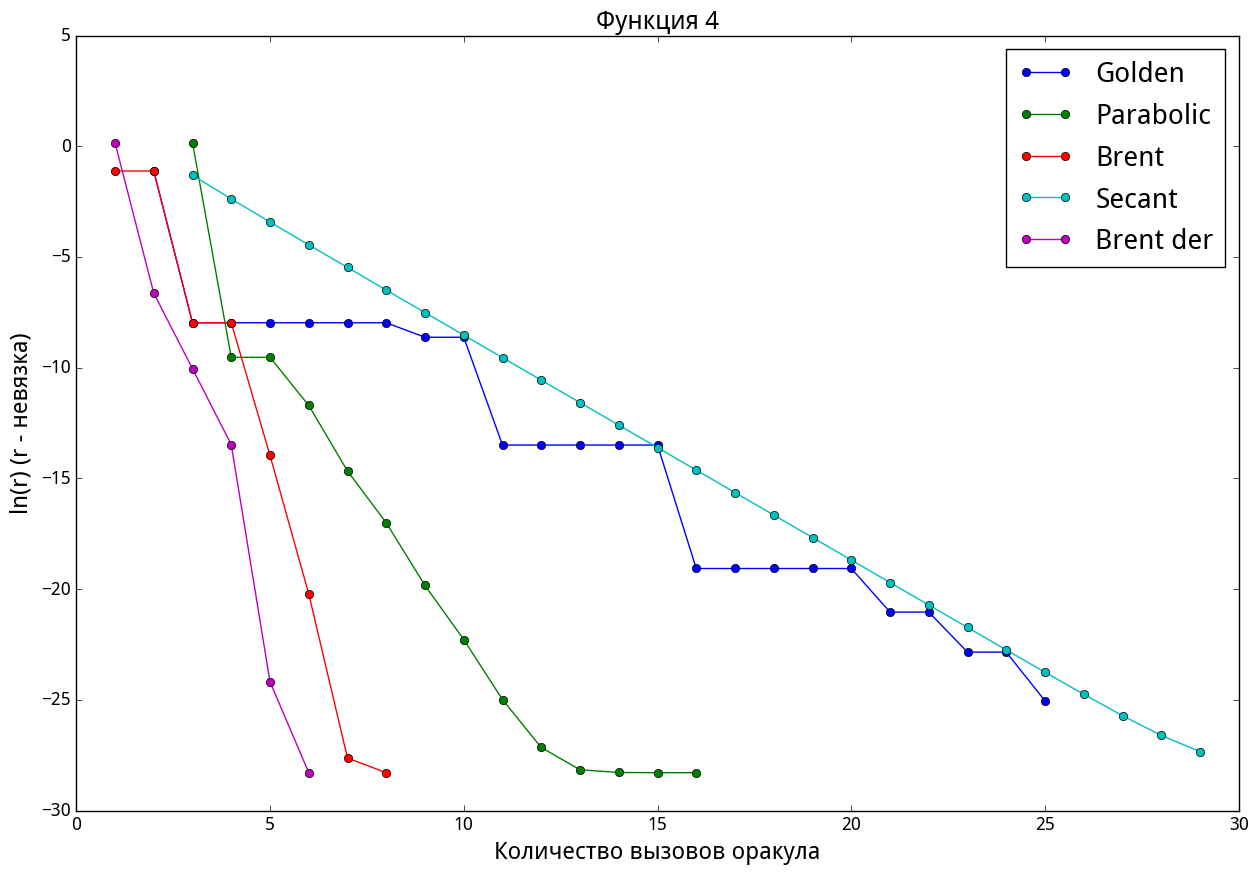
\includegraphics[width=\picwidth]{pics/fun4_der.png}\end{center}

        \newpage

        \textbf{Функция 5}

        \begin{center}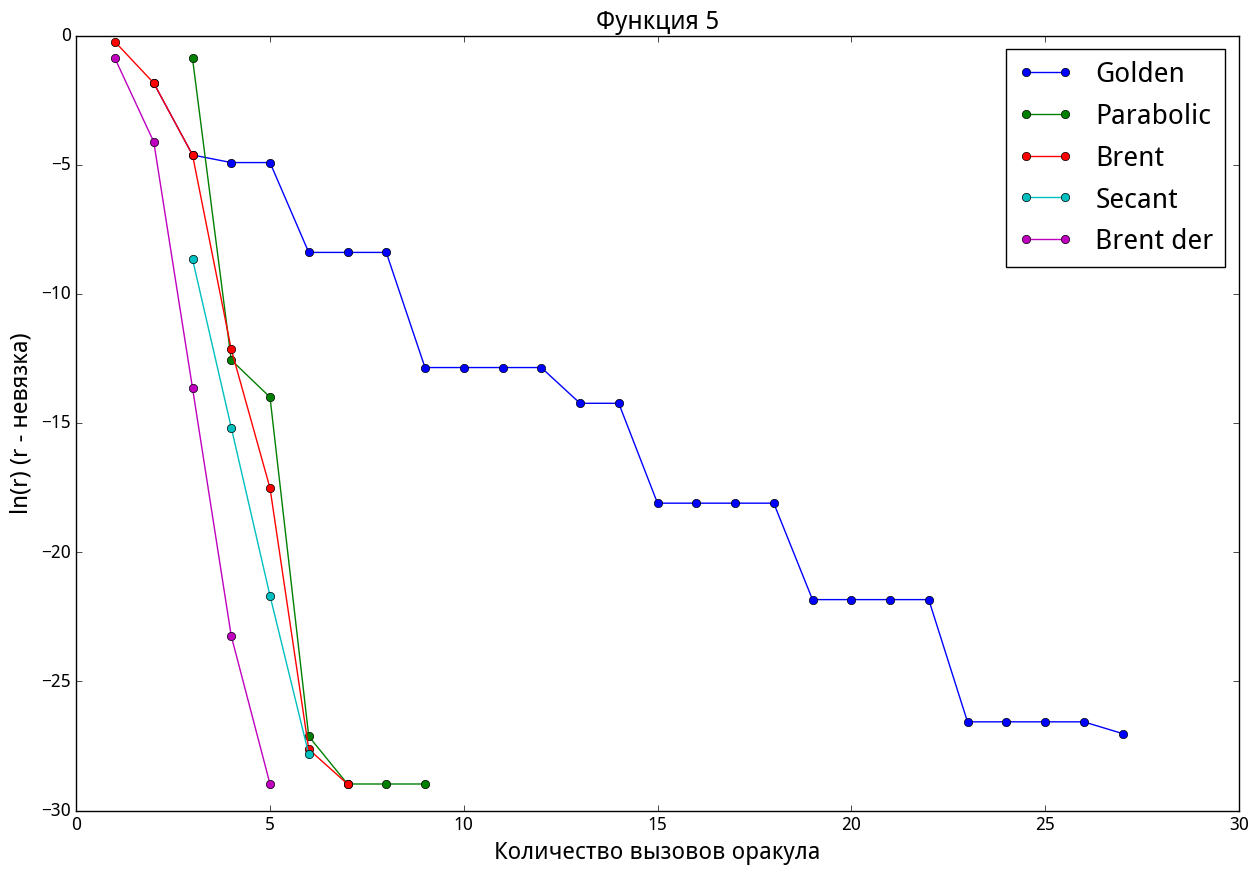
\includegraphics[width=\picwidth]{pics/fun5_der.png}\end{center}

        На всех графиках видно, что метод секущих сходится суперлинейно, но за большое количество итераций в общем случае. Метод Брента с производной тоже сходится суперлинейно, но в отличии от метода секущих, сходится быстрее. И в целом метод Брента с производной сходится быстрее остальных методов.

        Метод секущих на разных функциях ведет себя по разному. Но есть функции, на которых метод сходится очень медленно. Примером такой функции может служить следующая экспоненциальная функция:

        $f(x) = e^x - Cx, \text{где } C > 0$

        Если взять границы достаточно большими, чтобы график был ``прямым'' до определенной точки, и далее резко вырос, то метод будет сходится за тысячи шагов. Проверим это:

        Пусть $C = 100, a = -5, b = 12$

        При таких условиях метод сошелся за 4850 шагов, что медленно. Также надо отметить, что метод сходится суперлинейно, что можно видеть на графике сходимости метода

        \def \picwidth {8.7cm}

        \begin{center}
            \begin{tabular}{c c}
                \textbf{График функции} & \textbf{График функции в масштабе} \\

                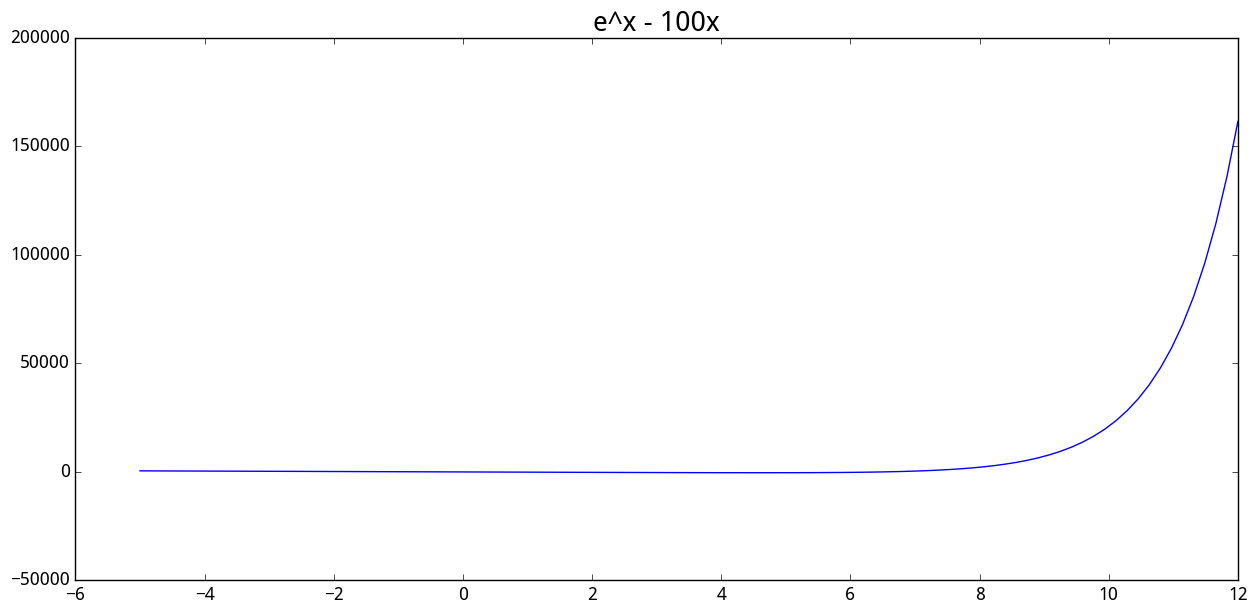
\includegraphics[width=\picwidth]{spec_sec.png} &
                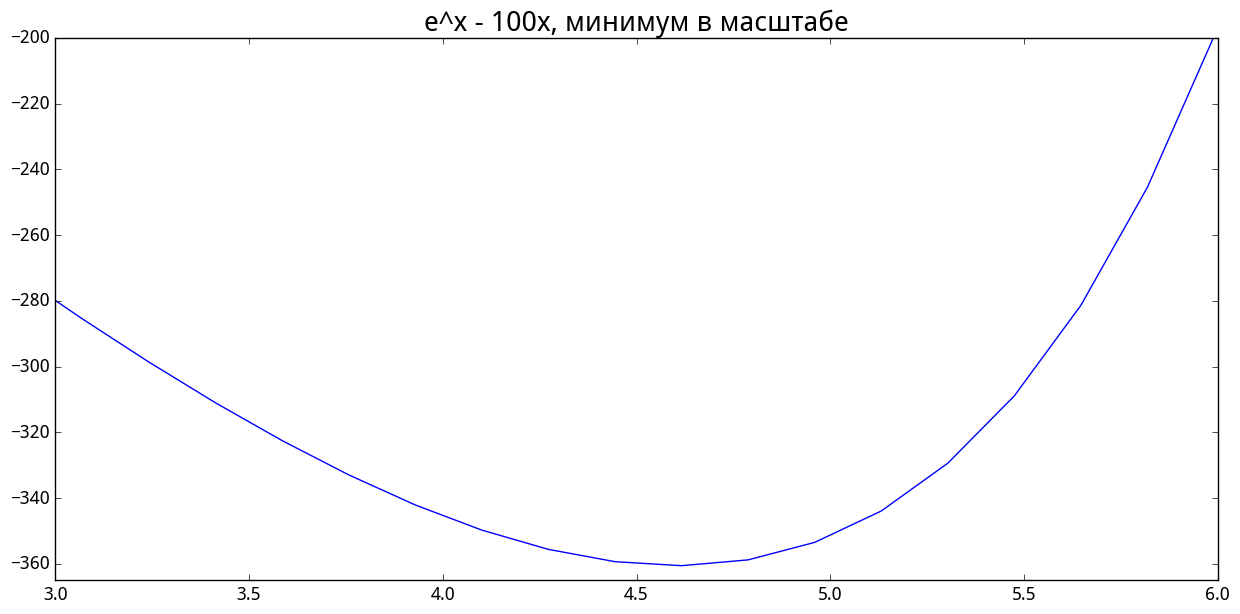
\includegraphics[width=\picwidth]{spec_sec_scaled.png} \\

                \textbf{График производной} & \textbf{График сходимости метода} \\

                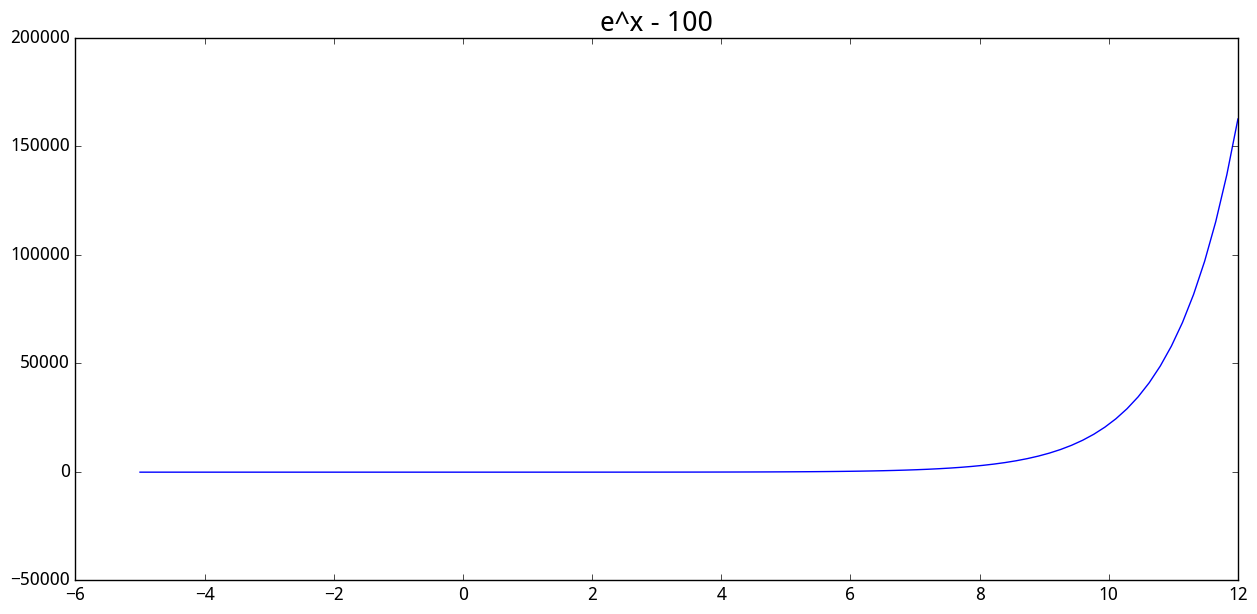
\includegraphics[width=\picwidth]{spec_sec_der.png} &
                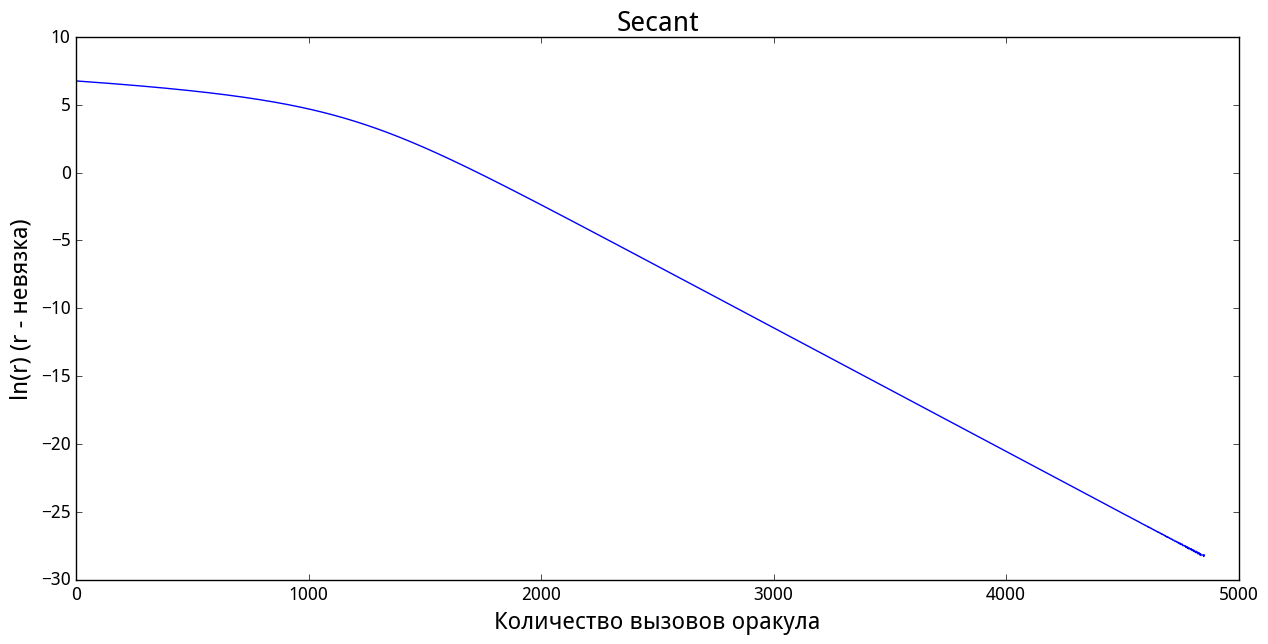
\includegraphics[width=\picwidth]{spec_sec_r.png} \\
            \end{tabular}
        \end{center}



    \section{Заключение}
        В работе мы сравнили методы точной оптимизации. Посмотрели их скорости сходимости и особенности. И в результате можно сказать, что самый быстрый метод без производной - метод Брента и самый быстрый метод с производной - метод Брента с производной. Эти методы не застревают в седловых точках и не находят максимум. Т.е. мы можем быть уверенными, что найдем локальный минимум функции (если он существует).

\end{document}
